\documentclass{book}
\usepackage[a4paper,top=2.5cm,bottom=2.5cm,left=2.5cm,right=2.5cm]{geometry}
\usepackage{makeidx}
\usepackage{natbib}
\usepackage{graphicx}
\usepackage{multicol}
\usepackage{float}
\usepackage{listings}
\usepackage{color}
\usepackage{ifthen}
\usepackage[table]{xcolor}
\usepackage{textcomp}
\usepackage{alltt}
\usepackage{ifpdf}
\ifpdf
\usepackage[pdftex,
            pagebackref=true,
            colorlinks=true,
            linkcolor=blue,
            unicode
           ]{hyperref}
\else
\usepackage[ps2pdf,
            pagebackref=true,
            colorlinks=true,
            linkcolor=blue,
            unicode
           ]{hyperref}
\usepackage{pspicture}
\fi
\usepackage[utf8]{inputenc}
\usepackage{mathptmx}
\usepackage[scaled=.90]{helvet}
\usepackage{courier}
\usepackage{sectsty}
\usepackage[titles]{tocloft}
\usepackage{doxygen}
\lstset{language=C++,inputencoding=utf8,basicstyle=\footnotesize,breaklines=true,breakatwhitespace=true,tabsize=4,numbers=left }
\makeindex
\setcounter{tocdepth}{3}
\renewcommand{\footrulewidth}{0.4pt}
\renewcommand{\familydefault}{\sfdefault}
\hfuzz=15pt
\setlength{\emergencystretch}{15pt}
\hbadness=750
\tolerance=750
\begin{document}
\hypersetup{pageanchor=false,citecolor=blue}
\begin{titlepage}
\vspace*{7cm}
\begin{center}
{\Large S\-A\-E Automated Shifter }\\
\vspace*{1cm}
{\large Generated by Doxygen 1.8.0}\\
\vspace*{0.5cm}
{\small Fri Apr 27 2012 08:25:19}\\
\end{center}
\end{titlepage}
\clearemptydoublepage
\pagenumbering{roman}
\tableofcontents
\clearemptydoublepage
\pagenumbering{arabic}
\hypersetup{pageanchor=true,citecolor=blue}
\chapter{Main Page}
\label{index}\hypertarget{index}{}\begin{DoxyAuthor}{Author}
Rocky Gray Jr.
\end{DoxyAuthor}
\hypertarget{index_intro}{}\section{Introduction}\label{index_intro}
Files used for this project\-:
\begin{DoxyItemize}
\item \hyperlink{_s_a_e___auto_shifter_8h}{S\-A\-E\-\_\-\-Auto\-Shifter.\-h}
\item \hyperlink{delay__rg_8h}{delay\-\_\-rg.\-h}
\item \hyperlink{main_8c}{main.\-c} 
\end{DoxyItemize}
\chapter{Module Index}
\section{Modules}
Here is a list of all modules\-:\begin{DoxyCompactList}
\item \contentsline{section}{Tachometer}{\pageref{group__tacho}}{}
\item \contentsline{section}{User Buttons}{\pageref{group__usr_btns}}{}
\end{DoxyCompactList}

\chapter{Data Structure Index}
\section{Data Structures}
Here are the data structures with brief descriptions\-:\begin{DoxyCompactList}
\item\contentsline{section}{\hyperlink{struct_gear}{Gear} }{\pageref{struct_gear}}{}
\item\contentsline{section}{\hyperlink{struct_tach}{Tach} }{\pageref{struct_tach}}{}
\item\contentsline{section}{\hyperlink{struct_usr___btns}{Usr\-\_\-\-Btns} }{\pageref{struct_usr___btns}}{}
\end{DoxyCompactList}

\chapter{File Index}
\section{File List}
Here is a list of all documented files with brief descriptions\-:\begin{DoxyCompactList}
\item\contentsline{section}{\hyperlink{defines_8h}{defines.\-h} \\*This file defines the pin mappings and critical definitions }{\pageref{defines_8h}}{}
\item\contentsline{section}{\hyperlink{delay__rg_8c}{delay\-\_\-rg.\-c} \\*This file defines delay functions that extend the usefullness of the avr-\/gcc delay functions }{\pageref{delay__rg_8c}}{}
\item\contentsline{section}{\hyperlink{delay__rg_8h}{delay\-\_\-rg.\-h} \\*This file defines delay functions that extend the usefullness of the avr-\/gcc delay functions }{\pageref{delay__rg_8h}}{}
\item\contentsline{section}{\hyperlink{main_8c}{main.\-c} \\*This file contains device specific initialization tasks and the main function }{\pageref{main_8c}}{}
\item\contentsline{section}{\hyperlink{_s_a_e___auto_shifter_8c}{S\-A\-E\-\_\-\-Auto\-Shifter.\-c} \\*This file defines the main task and I\-S\-Rs }{\pageref{_s_a_e___auto_shifter_8c}}{}
\item\contentsline{section}{\hyperlink{_s_a_e___auto_shifter_8h}{S\-A\-E\-\_\-\-Auto\-Shifter.\-h} \\*This header file contains constant definitions and function prototypes }{\pageref{_s_a_e___auto_shifter_8h}}{}
\item\contentsline{section}{{\bfseries serial.\-h} }{\pageref{serial_8h}}{}
\end{DoxyCompactList}

\chapter{Module Documentation}
\hypertarget{group__tacho}{\section{Tachometer}
\label{group__tacho}\index{Tachometer@{Tachometer}}
}
\subsection*{Data Structures}
\begin{DoxyCompactItemize}
\item 
struct \hyperlink{struct_tach}{Tach}
\end{DoxyCompactItemize}
\subsection*{Functions}
\begin{DoxyCompactItemize}
\item 
void \hyperlink{group__tacho_ga8746e3cc762f3153c2889e07dbb6ece0}{update\-\_\-ave\-\_\-rpms} ()
\item 
uint16\-\_\-t \hyperlink{group__tacho_gaa71ed50a06812b35c553b2291460396e}{average\-\_\-rpms} ()
\item 
\hypertarget{group__tacho_ga962c04c1da2810dd1602a83f649a454e}{uint16\-\_\-t {\bfseries cur\-\_\-rpms} ()}\label{group__tacho_ga962c04c1da2810dd1602a83f649a454e}

\end{DoxyCompactItemize}
\subsection*{Variables}
\begin{DoxyCompactItemize}
\item 
\hypertarget{group__tacho_ga3920911d3598cb499db825e8cb9adcad}{\hyperlink{struct_tach}{Tach} \hyperlink{group__tacho_ga3920911d3598cb499db825e8cb9adcad}{tach}}\label{group__tacho_ga3920911d3598cb499db825e8cb9adcad}

\begin{DoxyCompactList}\small\item\em Tachometer object. \end{DoxyCompactList}\end{DoxyCompactItemize}


\subsection{Detailed Description}
Holds the tach pulses and rpm conversion. {\ttfamily rpms} update at \hyperlink{defines_8h_a2f78c07e3b43ef498e926a39eff06b04}{T\-I\-M\-E\-R1\-\_\-\-F\-R\-E\-Q} 

\subsection{Function Documentation}
\hypertarget{group__tacho_gaa71ed50a06812b35c553b2291460396e}{\index{Tachometer@{Tachometer}!average\-\_\-rpms@{average\-\_\-rpms}}
\index{average\-\_\-rpms@{average\-\_\-rpms}!Tachometer@{Tachometer}}
\subsubsection[{average\-\_\-rpms}]{\setlength{\rightskip}{0pt plus 5cm}uint16\-\_\-t {\bf average\-\_\-rpms} (
\begin{DoxyParamCaption}
{}
\end{DoxyParamCaption}
)\hspace{0.3cm}{\ttfamily  \mbox{[}inline\mbox{]}}}}\label{group__tacho_gaa71ed50a06812b35c553b2291460396e}
\hyperlink{group__tacho_gaa71ed50a06812b35c553b2291460396e}{average\-\_\-rpms()} Returns the \hyperlink{struct_tach}{Tach}'s average rpm variable \hypertarget{group__tacho_ga8746e3cc762f3153c2889e07dbb6ece0}{\index{Tachometer@{Tachometer}!update\-\_\-ave\-\_\-rpms@{update\-\_\-ave\-\_\-rpms}}
\index{update\-\_\-ave\-\_\-rpms@{update\-\_\-ave\-\_\-rpms}!Tachometer@{Tachometer}}
\subsubsection[{update\-\_\-ave\-\_\-rpms}]{\setlength{\rightskip}{0pt plus 5cm}void {\bf update\-\_\-ave\-\_\-rpms} (
\begin{DoxyParamCaption}
{}
\end{DoxyParamCaption}
)\hspace{0.3cm}{\ttfamily  \mbox{[}inline\mbox{]}}}}\label{group__tacho_ga8746e3cc762f3153c2889e07dbb6ece0}
\hyperlink{group__tacho_ga8746e3cc762f3153c2889e07dbb6ece0}{update\-\_\-ave\-\_\-rpms()} Updates the \hyperlink{struct_tach}{Tach} rpm variable 
\hypertarget{group__usr_btns}{\section{User Buttons}
\label{group__usr_btns}\index{User Buttons@{User Buttons}}
}
\subsection*{Data Structures}
\begin{DoxyCompactItemize}
\item 
struct \hyperlink{struct_usr___btns}{Usr\-\_\-\-Btns}
\end{DoxyCompactItemize}
\subsection*{Functions}
\begin{DoxyCompactItemize}
\item 
uint8\-\_\-t \hyperlink{group__usr_btns_ga12edd371195cb085c440d64794fdf9ea}{btn\-\_\-state} (\hyperlink{struct_usr___btns}{Usr\-\_\-\-Btns} $\ast$u\-\_\-btn)
\item 
uint16\-\_\-t \hyperlink{group__usr_btns_ga10ac2ecdef1d96d9ef177f948817bbb3}{btn\-\_\-count} (\hyperlink{struct_usr___btns}{Usr\-\_\-\-Btns} $\ast$u\-\_\-btn)
\item 
\hypertarget{group__usr_btns_ga2f0699e265a6cc26a98e3470366b5cda}{uint8\-\_\-t {\bfseries on\-Release} (\hyperlink{struct_usr___btns}{Usr\-\_\-\-Btns} $\ast$btn)}\label{group__usr_btns_ga2f0699e265a6cc26a98e3470366b5cda}

\end{DoxyCompactItemize}
\subsection*{Variables}
\begin{DoxyCompactItemize}
\item 
\hypertarget{group__usr_btns_ga18ee634a9df9ed1ca0c7af2e021cec0f}{\hyperlink{struct_usr___btns}{Usr\-\_\-\-Btns} \hyperlink{group__usr_btns_ga18ee634a9df9ed1ca0c7af2e021cec0f}{up\-\_\-shift}}\label{group__usr_btns_ga18ee634a9df9ed1ca0c7af2e021cec0f}

\begin{DoxyCompactList}\small\item\em Upshift button. \end{DoxyCompactList}\item 
\hypertarget{group__usr_btns_gafd0b4b5ca080e04e71e4308414dc58ed}{\hyperlink{struct_usr___btns}{Usr\-\_\-\-Btns} \hyperlink{group__usr_btns_gafd0b4b5ca080e04e71e4308414dc58ed}{dn\-\_\-shift}}\label{group__usr_btns_gafd0b4b5ca080e04e71e4308414dc58ed}

\begin{DoxyCompactList}\small\item\em Downshift button. \end{DoxyCompactList}\end{DoxyCompactItemize}


\subsection{Detailed Description}
The states of the buttons, debounce values, and related functions. 

\subsection{Function Documentation}
\hypertarget{group__usr_btns_ga10ac2ecdef1d96d9ef177f948817bbb3}{\index{User Buttons@{User Buttons}!btn\-\_\-count@{btn\-\_\-count}}
\index{btn\-\_\-count@{btn\-\_\-count}!User Buttons@{User Buttons}}
\subsubsection[{btn\-\_\-count}]{\setlength{\rightskip}{0pt plus 5cm}uint16\-\_\-t {\bf btn\-\_\-count} (
\begin{DoxyParamCaption}
\item[{{\bf Usr\-\_\-\-Btns} $\ast$}]{u\-\_\-btn}
\end{DoxyParamCaption}
)\hspace{0.3cm}{\ttfamily  \mbox{[}inline\mbox{]}}}}\label{group__usr_btns_ga10ac2ecdef1d96d9ef177f948817bbb3}
btn\-\_\-cout()

\begin{DoxyReturn}{Returns}
the press {\ttfamily count} of {\ttfamily u\-\_\-btn} 
\end{DoxyReturn}
\hypertarget{group__usr_btns_ga12edd371195cb085c440d64794fdf9ea}{\index{User Buttons@{User Buttons}!btn\-\_\-state@{btn\-\_\-state}}
\index{btn\-\_\-state@{btn\-\_\-state}!User Buttons@{User Buttons}}
\subsubsection[{btn\-\_\-state}]{\setlength{\rightskip}{0pt plus 5cm}uint8\-\_\-t {\bf btn\-\_\-state} (
\begin{DoxyParamCaption}
\item[{{\bf Usr\-\_\-\-Btns} $\ast$}]{u\-\_\-btn}
\end{DoxyParamCaption}
)\hspace{0.3cm}{\ttfamily  \mbox{[}inline\mbox{]}}}}\label{group__usr_btns_ga12edd371195cb085c440d64794fdf9ea}
\hyperlink{group__usr_btns_ga12edd371195cb085c440d64794fdf9ea}{btn\-\_\-state()}

\begin{DoxyReturn}{Returns}
the {\ttfamily state} of {\ttfamily u\-\_\-btn} 
\end{DoxyReturn}

\chapter{Data Structure Documentation}
\hypertarget{struct_gear}{\section{Gear Struct Reference}
\label{struct_gear}\index{Gear@{Gear}}
}


{\ttfamily \#include $<$S\-A\-E\-\_\-\-Auto\-Shifter.\-h$>$}



Collaboration diagram for Gear\-:\nopagebreak
\begin{figure}[H]
\begin{center}
\leavevmode
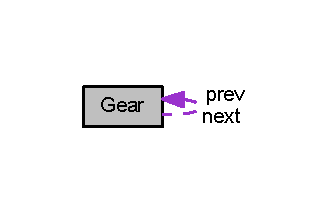
\includegraphics[width=157pt]{struct_gear__coll__graph}
\end{center}
\end{figure}
\subsection*{Data Fields}
\begin{DoxyCompactItemize}
\item 
\hypertarget{struct_gear_af2d4d012a23bd6c3c754ac100160dc4b}{uint8\-\_\-t \hyperlink{struct_gear_af2d4d012a23bd6c3c754ac100160dc4b}{g\-\_\-num}}\label{struct_gear_af2d4d012a23bd6c3c754ac100160dc4b}

\begin{DoxyCompactList}\small\item\em Number of the \hyperlink{struct_gear}{Gear}. \end{DoxyCompactList}\item 
\hypertarget{struct_gear_aa652deac3cdb2d1e72f92da6bfc6e2c3}{uint16\-\_\-t \hyperlink{struct_gear_aa652deac3cdb2d1e72f92da6bfc6e2c3}{lower\-B}}\label{struct_gear_aa652deac3cdb2d1e72f92da6bfc6e2c3}

\begin{DoxyCompactList}\small\item\em Lower bound of \hyperlink{struct_gear}{Gear}. \end{DoxyCompactList}\item 
\hypertarget{struct_gear_a617a595c6b471c4d9a82bb4fc78e4d1b}{uint16\-\_\-t \hyperlink{struct_gear_a617a595c6b471c4d9a82bb4fc78e4d1b}{upper\-B}}\label{struct_gear_a617a595c6b471c4d9a82bb4fc78e4d1b}

\begin{DoxyCompactList}\small\item\em Upper bound of \hyperlink{struct_gear}{Gear}. \end{DoxyCompactList}\item 
\hypertarget{struct_gear_a5bbd2050715b3f8755b9b2a3cb103032}{struct \hyperlink{struct_gear}{Gear} $\ast$ \hyperlink{struct_gear_a5bbd2050715b3f8755b9b2a3cb103032}{prev}}\label{struct_gear_a5bbd2050715b3f8755b9b2a3cb103032}

\begin{DoxyCompactList}\small\item\em Previous gear. \end{DoxyCompactList}\item 
\hypertarget{struct_gear_a2a049b2f216c8222bd6d4ddbae567ca6}{struct \hyperlink{struct_gear}{Gear} $\ast$ \hyperlink{struct_gear_a2a049b2f216c8222bd6d4ddbae567ca6}{next}}\label{struct_gear_a2a049b2f216c8222bd6d4ddbae567ca6}

\begin{DoxyCompactList}\small\item\em Next gear. \end{DoxyCompactList}\end{DoxyCompactItemize}


\subsection{Detailed Description}
defgroup gears Gears Defines the gear structure and related functions. 

The documentation for this struct was generated from the following file\-:\begin{DoxyCompactItemize}
\item 
\hyperlink{_s_a_e___auto_shifter_8h}{S\-A\-E\-\_\-\-Auto\-Shifter.\-h}\end{DoxyCompactItemize}

\hypertarget{struct_tach}{\section{Tach Struct Reference}
\label{struct_tach}\index{Tach@{Tach}}
}
\subsection*{Data Fields}
\begin{DoxyCompactItemize}
\item 
\hypertarget{struct_tach_a1a8d74dba687155486d4c8b8e135596b}{uint16\-\_\-t {\bfseries pulse}}\label{struct_tach_a1a8d74dba687155486d4c8b8e135596b}

\item 
\hypertarget{struct_tach_a5d1fadcd5a3332f34e86e5f999e84e0c}{uint16\-\_\-t {\bfseries rpms}}\label{struct_tach_a5d1fadcd5a3332f34e86e5f999e84e0c}

\item 
\hypertarget{struct_tach_a319acaf9f8de490483e8ff5d5cb4d408}{uint8\-\_\-t {\bfseries index}}\label{struct_tach_a319acaf9f8de490483e8ff5d5cb4d408}

\item 
\hypertarget{struct_tach_a52bbe734dfee43e0550d14084a2a6f47}{uint16\-\_\-t {\bfseries rpms\-\_\-hist} \mbox{[}\hyperlink{defines_8h_aaf14a33c47932dfc82df5f2b09444c71}{R\-P\-M\-\_\-\-H\-I\-S\-T\-\_\-\-L\-E\-N}\mbox{]}}\label{struct_tach_a52bbe734dfee43e0550d14084a2a6f47}

\item 
\hypertarget{struct_tach_a8653bd5b693ebfe1a8dbde8bd5d9b48e}{uint16\-\_\-t {\bfseries ave}}\label{struct_tach_a8653bd5b693ebfe1a8dbde8bd5d9b48e}

\end{DoxyCompactItemize}


The documentation for this struct was generated from the following file\-:\begin{DoxyCompactItemize}
\item 
\hyperlink{_s_a_e___auto_shifter_8h}{S\-A\-E\-\_\-\-Auto\-Shifter.\-h}\end{DoxyCompactItemize}

\hypertarget{struct_usr___btns}{\section{Usr\-\_\-\-Btns Struct Reference}
\label{struct_usr___btns}\index{Usr\-\_\-\-Btns@{Usr\-\_\-\-Btns}}
}
\subsection*{Data Fields}
\begin{DoxyCompactItemize}
\item 
\hypertarget{struct_usr___btns_a8c0a3343e556825e6b6c30b0e050978b}{uint8\-\_\-t \hyperlink{struct_usr___btns_a8c0a3343e556825e6b6c30b0e050978b}{state}}\label{struct_usr___btns_a8c0a3343e556825e6b6c30b0e050978b}

\begin{DoxyCompactList}\small\item\em Button state. Either \hyperlink{defines_8h_a654adff3c664f27f0b29c24af818dd26}{P\-R\-E\-S\-S\-E\-D} or \hyperlink{defines_8h_ad74b7f5218b46c8332cd531df7178d45}{R\-E\-L\-E\-A\-S\-E\-D}. \end{DoxyCompactList}\item 
\hypertarget{struct_usr___btns_a8275ba5ecf7ab28a7eba0382ddf91577}{uint16\-\_\-t \hyperlink{struct_usr___btns_a8275ba5ecf7ab28a7eba0382ddf91577}{count}}\label{struct_usr___btns_a8275ba5ecf7ab28a7eba0382ddf91577}

\begin{DoxyCompactList}\small\item\em Button Press count. \end{DoxyCompactList}\end{DoxyCompactItemize}


The documentation for this struct was generated from the following file\-:\begin{DoxyCompactItemize}
\item 
\hyperlink{_s_a_e___auto_shifter_8h}{S\-A\-E\-\_\-\-Auto\-Shifter.\-h}\end{DoxyCompactItemize}

\chapter{File Documentation}
\hypertarget{defines_8h}{\section{defines.\-h File Reference}
\label{defines_8h}\index{defines.\-h@{defines.\-h}}
}


This file defines the pin mappings and critical definitions.  


{\ttfamily \#include $<$avr/io.\-h$>$}\\*
Include dependency graph for defines.\-h\-:\nopagebreak
\begin{figure}[H]
\begin{center}
\leavevmode
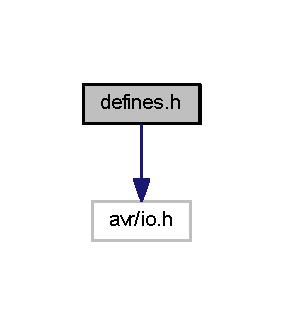
\includegraphics[width=136pt]{defines_8h__incl}
\end{center}
\end{figure}
This graph shows which files directly or indirectly include this file\-:\nopagebreak
\begin{figure}[H]
\begin{center}
\leavevmode
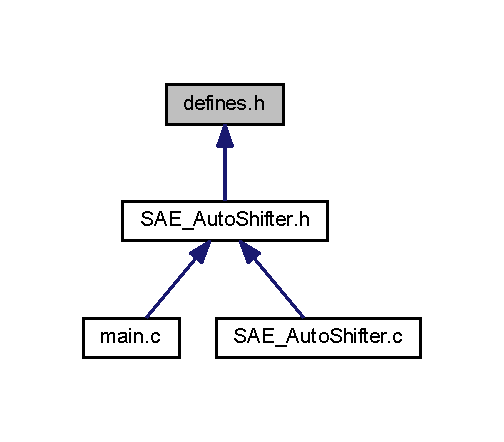
\includegraphics[width=242pt]{defines_8h__dep__incl}
\end{center}
\end{figure}
\subsection*{Defines}
\begin{Indent}{\bf User Input Defines}\par
\begin{DoxyCompactItemize}
\item 
\hypertarget{defines_8h_a0f1aed08f5269f1bddc80c20ecaec0be}{\#define \hyperlink{defines_8h_a0f1aed08f5269f1bddc80c20ecaec0be}{B\-T\-N\-\_\-\-I\-P\-\_\-\-D\-D\-R}~D\-D\-R\-D}\label{defines_8h_a0f1aed08f5269f1bddc80c20ecaec0be}

\begin{DoxyCompactList}\small\item\em Button input D\-D\-R. \end{DoxyCompactList}\item 
\hypertarget{defines_8h_a6ac943017d31877e3b86387e14c9b006}{\#define \hyperlink{defines_8h_a6ac943017d31877e3b86387e14c9b006}{B\-T\-N\-\_\-\-I\-P\-\_\-\-P\-O\-R\-T}~P\-O\-R\-T\-D}\label{defines_8h_a6ac943017d31877e3b86387e14c9b006}

\begin{DoxyCompactList}\small\item\em Button input Port. \end{DoxyCompactList}\item 
\hypertarget{defines_8h_a220b3ddb5e9bac9ed273e011f267a536}{\#define \hyperlink{defines_8h_a220b3ddb5e9bac9ed273e011f267a536}{B\-T\-N\-\_\-\-I\-P\-\_\-\-P\-I\-N}~P\-I\-N\-D}\label{defines_8h_a220b3ddb5e9bac9ed273e011f267a536}

\begin{DoxyCompactList}\small\item\em Button input Port Pins. \end{DoxyCompactList}\item 
\hypertarget{defines_8h_ac4a361c6ecdb8ef9a4c7a7253fa0feb8}{\#define \hyperlink{defines_8h_ac4a361c6ecdb8ef9a4c7a7253fa0feb8}{U\-S\-H\-I\-F\-T\-\_\-\-P\-I\-N}~P\-D4}\label{defines_8h_ac4a361c6ecdb8ef9a4c7a7253fa0feb8}

\begin{DoxyCompactList}\small\item\em Upshift pin\par
 Connect to Digital Pin 4. \end{DoxyCompactList}\item 
\hypertarget{defines_8h_a7f2aeb6091a43ad2b243e35a521ec5b0}{\#define \hyperlink{defines_8h_a7f2aeb6091a43ad2b243e35a521ec5b0}{D\-S\-H\-I\-F\-T\-\_\-\-P\-I\-N}~P\-D5}\label{defines_8h_a7f2aeb6091a43ad2b243e35a521ec5b0}

\begin{DoxyCompactList}\small\item\em Downshift pin\par
 Connect to Digital Pin 5. \end{DoxyCompactList}\item 
\hypertarget{defines_8h_a60210b83e17d109c8071e39f97743e55}{\#define \hyperlink{defines_8h_a60210b83e17d109c8071e39f97743e55}{S\-E\-M\-I\-A\-U\-T\-O\-\_\-\-P\-I\-N}~P\-D6}\label{defines_8h_a60210b83e17d109c8071e39f97743e55}

\begin{DoxyCompactList}\small\item\em Mode pin\par
 Connect to Digital Pin 6. \end{DoxyCompactList}\item 
\hypertarget{defines_8h_a73819d778660496733ab530f442f7ea3}{\#define \hyperlink{defines_8h_a73819d778660496733ab530f442f7ea3}{A\-U\-T\-O\-M\-A\-T\-I\-C\-\_\-\-P\-I\-N}~P\-D7}\label{defines_8h_a73819d778660496733ab530f442f7ea3}

\begin{DoxyCompactList}\small\item\em Mode pin\par
 Connect to Digital Pin 7. \end{DoxyCompactList}\item 
\hypertarget{defines_8h_ad74b7f5218b46c8332cd531df7178d45}{\#define \hyperlink{defines_8h_ad74b7f5218b46c8332cd531df7178d45}{R\-E\-L\-E\-A\-S\-E\-D}~0}\label{defines_8h_ad74b7f5218b46c8332cd531df7178d45}

\begin{DoxyCompactList}\small\item\em Button is released. \end{DoxyCompactList}\item 
\hypertarget{defines_8h_a654adff3c664f27f0b29c24af818dd26}{\#define \hyperlink{defines_8h_a654adff3c664f27f0b29c24af818dd26}{P\-R\-E\-S\-S\-E\-D}~1}\label{defines_8h_a654adff3c664f27f0b29c24af818dd26}

\begin{DoxyCompactList}\small\item\em Button is pressed. \end{DoxyCompactList}\item 
\hypertarget{defines_8h_af4807ecc777e3a39d6c4da1e158594bf}{\#define \hyperlink{defines_8h_af4807ecc777e3a39d6c4da1e158594bf}{D\-B\-\_\-\-D\-E\-L\-A\-Y}~200}\label{defines_8h_af4807ecc777e3a39d6c4da1e158594bf}

\begin{DoxyCompactList}\small\item\em Debounce delay (ms) \end{DoxyCompactList}\item 
\hypertarget{defines_8h_a6f53fbd627478c7f56cdb17b5aa3ff44}{\#define \hyperlink{defines_8h_a6f53fbd627478c7f56cdb17b5aa3ff44}{A\-D\-C\-\_\-\-D\-D\-R}~D\-D\-R\-C}\label{defines_8h_a6f53fbd627478c7f56cdb17b5aa3ff44}

\begin{DoxyCompactList}\small\item\em A\-D\-C D\-D\-R. \end{DoxyCompactList}\item 
\hypertarget{defines_8h_a1c6ce969ab3d12ac37f62c399a1e02c1}{\#define \hyperlink{defines_8h_a1c6ce969ab3d12ac37f62c399a1e02c1}{A\-D\-C\-\_\-\-P\-O\-R\-T}~P\-O\-R\-T\-C}\label{defines_8h_a1c6ce969ab3d12ac37f62c399a1e02c1}

\begin{DoxyCompactList}\small\item\em A\-D\-C Port. \end{DoxyCompactList}\item 
\hypertarget{defines_8h_af458889265f213625129e2dd0707a69b}{\#define \hyperlink{defines_8h_af458889265f213625129e2dd0707a69b}{A\-D\-C\-\_\-\-P\-I\-N}~P\-I\-N\-C}\label{defines_8h_af458889265f213625129e2dd0707a69b}

\begin{DoxyCompactList}\small\item\em A\-D\-C Port Pins. \end{DoxyCompactList}\item 
\hypertarget{defines_8h_a5fa15e6af6db071b58a794dd279d3e65}{\#define \hyperlink{defines_8h_a5fa15e6af6db071b58a794dd279d3e65}{G\-A\-S\-\_\-\-P\-E\-D\-A\-L}~P\-C0}\label{defines_8h_a5fa15e6af6db071b58a794dd279d3e65}

\begin{DoxyCompactList}\small\item\em Gas pedal input pin. \end{DoxyCompactList}\end{DoxyCompactItemize}
\end{Indent}
\begin{Indent}{\bf Solenoid Defines}\par
\begin{DoxyCompactItemize}
\item 
\hypertarget{defines_8h_a3ca3b069d7464c17c03b5b1e7da788fd}{\#define \hyperlink{defines_8h_a3ca3b069d7464c17c03b5b1e7da788fd}{S\-O\-L\-E\-N\-\_\-\-O\-P\-\_\-\-D\-D\-R}~D\-D\-R\-B}\label{defines_8h_a3ca3b069d7464c17c03b5b1e7da788fd}

\begin{DoxyCompactList}\small\item\em Solenoid output D\-D\-R. \end{DoxyCompactList}\item 
\hypertarget{defines_8h_a4ad600582a951bdd4b75311388dc6ae7}{\#define \hyperlink{defines_8h_a4ad600582a951bdd4b75311388dc6ae7}{S\-O\-L\-E\-N\-\_\-\-O\-P\-\_\-\-P\-O\-R\-T}~P\-O\-R\-T\-B}\label{defines_8h_a4ad600582a951bdd4b75311388dc6ae7}

\begin{DoxyCompactList}\small\item\em Solenoid output Port. \end{DoxyCompactList}\item 
\hypertarget{defines_8h_a473a2cf5e606d18feb583ec4749a49ea}{\#define \hyperlink{defines_8h_a473a2cf5e606d18feb583ec4749a49ea}{S\-O\-L\-E\-N\-\_\-\-O\-P\-\_\-\-P\-I\-N}~P\-I\-N\-B}\label{defines_8h_a473a2cf5e606d18feb583ec4749a49ea}

\begin{DoxyCompactList}\small\item\em Solenoid output Port Pins. \end{DoxyCompactList}\item 
\hypertarget{defines_8h_aeacdff688cfbf944da03e3c972f878f0}{\#define \hyperlink{defines_8h_aeacdff688cfbf944da03e3c972f878f0}{S\-O\-L\-E\-N\-\_\-\-U\-P}~P\-B1}\label{defines_8h_aeacdff688cfbf944da03e3c972f878f0}

\begin{DoxyCompactList}\small\item\em Solenoid Up, pulls solenoid in. \end{DoxyCompactList}\item 
\hypertarget{defines_8h_ae38dab54770629f5f2b7975164123353}{\#define \hyperlink{defines_8h_ae38dab54770629f5f2b7975164123353}{S\-O\-L\-E\-N\-\_\-\-D\-N}~P\-B2}\label{defines_8h_ae38dab54770629f5f2b7975164123353}

\begin{DoxyCompactList}\small\item\em Solenoid Down, pushes solenoid out. \end{DoxyCompactList}\item 
\hypertarget{defines_8h_a93d7b661115e27ae25e9535e7035d79e}{\#define \hyperlink{defines_8h_a93d7b661115e27ae25e9535e7035d79e}{S\-O\-L\-E\-N\-\_\-\-D\-L\-Y}~200}\label{defines_8h_a93d7b661115e27ae25e9535e7035d79e}

\begin{DoxyCompactList}\small\item\em Amount of time to hold Solenoid. \end{DoxyCompactList}\end{DoxyCompactItemize}
\end{Indent}
\begin{Indent}{\bf E\-C\-U Defines}\par
\begin{DoxyCompactItemize}
\item 
\hypertarget{defines_8h_adcf75600abb29c4672e4fe8ab1a1cebf}{\#define \hyperlink{defines_8h_adcf75600abb29c4672e4fe8ab1a1cebf}{E\-C\-U\-\_\-\-D\-D\-R}~D\-D\-R\-D}\label{defines_8h_adcf75600abb29c4672e4fe8ab1a1cebf}

\begin{DoxyCompactList}\small\item\em Tachometer input D\-D\-R. \end{DoxyCompactList}\item 
\hypertarget{defines_8h_af933c954441ed711d862e64baa777e53}{\#define \hyperlink{defines_8h_af933c954441ed711d862e64baa777e53}{E\-C\-U\-\_\-\-P\-O\-R\-T}~P\-O\-R\-T\-D}\label{defines_8h_af933c954441ed711d862e64baa777e53}

\begin{DoxyCompactList}\small\item\em Tachometer input Port. \end{DoxyCompactList}\item 
\hypertarget{defines_8h_abf1d20db3cddde61117882c98451e5b6}{\#define \hyperlink{defines_8h_abf1d20db3cddde61117882c98451e5b6}{E\-C\-U\-\_\-\-P\-I\-N}~P\-I\-N\-D}\label{defines_8h_abf1d20db3cddde61117882c98451e5b6}

\begin{DoxyCompactList}\small\item\em Tachometer input Port Pins. \end{DoxyCompactList}\item 
\hypertarget{defines_8h_af84d0d7a25d38271813b650eeb6a4228}{\#define \hyperlink{defines_8h_af84d0d7a25d38271813b650eeb6a4228}{T\-A\-C\-H\-\_\-\-P\-I\-N}~P\-D2}\label{defines_8h_af84d0d7a25d38271813b650eeb6a4228}

\begin{DoxyCompactList}\small\item\em Tachometer pin\par
 Connect to Digital Pin 2. \end{DoxyCompactList}\item 
\hypertarget{defines_8h_a8759f4bc82fbb897f8e934158d2acc76}{\#define \hyperlink{defines_8h_a8759f4bc82fbb897f8e934158d2acc76}{I\-G\-N\-I\-T\-I\-O\-N\-\_\-\-I\-N\-T}~P\-D3}\label{defines_8h_a8759f4bc82fbb897f8e934158d2acc76}

\begin{DoxyCompactList}\small\item\em Ignition interrupt pin\par
 Connect to Digital Pin 3. \end{DoxyCompactList}\item 
\hypertarget{defines_8h_afffe9f2e5a46dd0430947cd1a9b80a63}{\#define \hyperlink{defines_8h_afffe9f2e5a46dd0430947cd1a9b80a63}{I\-G\-N\-I\-T\-I\-O\-N\-\_\-\-D\-L\-Y}~300}\label{defines_8h_afffe9f2e5a46dd0430947cd1a9b80a63}

\begin{DoxyCompactList}\small\item\em Ignition kill duration. \end{DoxyCompactList}\item 
\hypertarget{defines_8h_aba70372cd9d0d4cfda5b901bb2226114}{\#define \hyperlink{defines_8h_aba70372cd9d0d4cfda5b901bb2226114}{P\-U\-L\-S\-E\-\_\-\-R\-O\-T}~2}\label{defines_8h_aba70372cd9d0d4cfda5b901bb2226114}

\begin{DoxyCompactList}\small\item\em Number of pulses per rotation. \end{DoxyCompactList}\item 
\hypertarget{defines_8h_aaf14a33c47932dfc82df5f2b09444c71}{\#define \hyperlink{defines_8h_aaf14a33c47932dfc82df5f2b09444c71}{R\-P\-M\-\_\-\-H\-I\-S\-T\-\_\-\-L\-E\-N}~10}\label{defines_8h_aaf14a33c47932dfc82df5f2b09444c71}

\begin{DoxyCompactList}\small\item\em Length of R\-P\-M history. \end{DoxyCompactList}\item 
\hypertarget{defines_8h_a03f0cc69336f88fcd5943808f19bab28}{\#define \hyperlink{defines_8h_a03f0cc69336f88fcd5943808f19bab28}{R\-P\-M\-\_\-\-M\-A\-X}~7000}\label{defines_8h_a03f0cc69336f88fcd5943808f19bab28}

\begin{DoxyCompactList}\small\item\em Maximum rpm for down shifting. \end{DoxyCompactList}\end{DoxyCompactItemize}
\end{Indent}
\begin{Indent}{\bf Timer Defines}\par
\begin{DoxyCompactItemize}
\item 
\hypertarget{defines_8h_abbc7611d058a56c043591fab1ffede31}{\#define \hyperlink{defines_8h_abbc7611d058a56c043591fab1ffede31}{T\-I\-M\-E\-R0\-\_\-\-F\-R\-E\-Q}~1000}\label{defines_8h_abbc7611d058a56c043591fab1ffede31}

\begin{DoxyCompactList}\small\item\em Button pin check frequency (Hz). \end{DoxyCompactList}\item 
\hypertarget{defines_8h_a42b5bcd9eeb1d25e27f7dffba04a1507}{\#define \hyperlink{defines_8h_a42b5bcd9eeb1d25e27f7dffba04a1507}{P\-R\-E\-S\-C\-A\-L\-E\-R0}~64}\label{defines_8h_a42b5bcd9eeb1d25e27f7dffba04a1507}

\begin{DoxyCompactList}\small\item\em Prescaler needed for Timer0. \end{DoxyCompactList}\item 
\hypertarget{defines_8h_a2f78c07e3b43ef498e926a39eff06b04}{\#define \hyperlink{defines_8h_a2f78c07e3b43ef498e926a39eff06b04}{T\-I\-M\-E\-R1\-\_\-\-F\-R\-E\-Q}~1}\label{defines_8h_a2f78c07e3b43ef498e926a39eff06b04}

\begin{DoxyCompactList}\small\item\em R\-P\-M sample frequency (Hz). \end{DoxyCompactList}\item 
\hypertarget{defines_8h_a8e5346fd5983419a0dbcbbc4995c7ea7}{\#define \hyperlink{defines_8h_a8e5346fd5983419a0dbcbbc4995c7ea7}{P\-R\-E\-S\-C\-A\-L\-E\-R1}~256}\label{defines_8h_a8e5346fd5983419a0dbcbbc4995c7ea7}

\begin{DoxyCompactList}\small\item\em Prescaler needed for Timer1. \end{DoxyCompactList}\end{DoxyCompactItemize}
\end{Indent}
\begin{Indent}{\bf L\-E\-D Defines}\par
\begin{DoxyCompactItemize}
\item 
\hypertarget{defines_8h_ae5ba1fb0b349f2a7f2fb82cb2cf39cbb}{\#define \hyperlink{defines_8h_ae5ba1fb0b349f2a7f2fb82cb2cf39cbb}{B\-O\-A\-R\-D\-\_\-\-D\-D\-R}~D\-D\-R\-B}\label{defines_8h_ae5ba1fb0b349f2a7f2fb82cb2cf39cbb}

\begin{DoxyCompactList}\small\item\em Board light D\-D\-R. \end{DoxyCompactList}\item 
\hypertarget{defines_8h_a538e637dc4c2e333b294814e381d9a75}{\#define \hyperlink{defines_8h_a538e637dc4c2e333b294814e381d9a75}{B\-O\-A\-R\-D\-\_\-\-P\-O\-R\-T}~P\-O\-R\-T\-B}\label{defines_8h_a538e637dc4c2e333b294814e381d9a75}

\begin{DoxyCompactList}\small\item\em Board light Port. \end{DoxyCompactList}\item 
\hypertarget{defines_8h_aae20f7b7253ad1be81ef8a486a7dfa8e}{\#define \hyperlink{defines_8h_aae20f7b7253ad1be81ef8a486a7dfa8e}{B\-O\-A\-R\-D\-\_\-\-P\-I\-N}~P\-I\-N\-B}\label{defines_8h_aae20f7b7253ad1be81ef8a486a7dfa8e}

\begin{DoxyCompactList}\small\item\em Board light Pin. \end{DoxyCompactList}\item 
\hypertarget{defines_8h_a5a54034c799f34b35663b774a715a581}{\#define \hyperlink{defines_8h_a5a54034c799f34b35663b774a715a581}{R\-O\-L\-L\-\_\-\-D\-E\-L\-A\-Y}~300}\label{defines_8h_a5a54034c799f34b35663b774a715a581}

\begin{DoxyCompactList}\small\item\em Roll time (ms) \end{DoxyCompactList}\item 
\hypertarget{defines_8h_a9ac61ad7c19d5a7d1f4cb1b45f41c7b1}{\#define \hyperlink{defines_8h_a9ac61ad7c19d5a7d1f4cb1b45f41c7b1}{B\-O\-A\-R\-D\-\_\-\-L\-I\-G\-H\-T}~P\-B5}\label{defines_8h_a9ac61ad7c19d5a7d1f4cb1b45f41c7b1}

\begin{DoxyCompactList}\small\item\em On board light. \end{DoxyCompactList}\end{DoxyCompactItemize}
\end{Indent}
\begin{Indent}{\bf Gear Defines}\par
\begin{DoxyCompactItemize}
\item 
\hypertarget{defines_8h_a33a107b04949dd6a51b20f625eeb8b75}{\#define \hyperlink{defines_8h_a33a107b04949dd6a51b20f625eeb8b75}{M\-A\-X\-\_\-\-G\-E\-A\-R\-S}~5}\label{defines_8h_a33a107b04949dd6a51b20f625eeb8b75}

\begin{DoxyCompactList}\small\item\em Maximum number of gears. \end{DoxyCompactList}\end{DoxyCompactItemize}
\end{Indent}


\subsection{Detailed Description}
This file defines the pin mappings and critical definitions. \begin{DoxyAuthor}{Author}
Rocky Gray Jr.
\end{DoxyAuthor}
\begin{DoxyDate}{Date}
3/27/2012 
\end{DoxyDate}

\hypertarget{delay__rg_8c}{\section{delay\-\_\-rg.\-c File Reference}
\label{delay__rg_8c}\index{delay\-\_\-rg.\-c@{delay\-\_\-rg.\-c}}
}


This file defines delay functions that extend the usefullness of the avr-\/gcc delay functions.  


{\ttfamily \#include \char`\"{}delay\-\_\-rg.\-h\char`\"{}}\\*
Include dependency graph for delay\-\_\-rg.\-c\-:\nopagebreak
\begin{figure}[H]
\begin{center}
\leavevmode
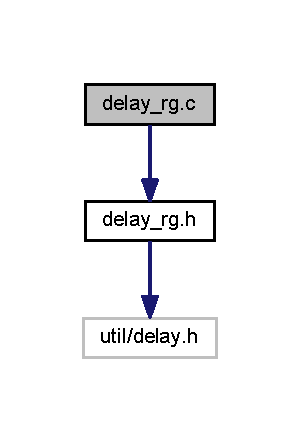
\includegraphics[width=144pt]{delay__rg_8c__incl}
\end{center}
\end{figure}
\subsection*{Functions}
\begin{DoxyCompactItemize}
\item 
void \hyperlink{delay__rg_8c_aa0dce6d249d81fb85b082273270ba710}{delay\-\_\-ms} (uint16\-\_\-t ms)
\begin{DoxyCompactList}\small\item\em Delays for {\ttfamily ms} milliseconds. \end{DoxyCompactList}\item 
void \hyperlink{delay__rg_8c_a58f9378c36dbb864c00f8c964c652173}{delay\-\_\-us} (uint16\-\_\-t us)
\begin{DoxyCompactList}\small\item\em Delays for {\ttfamily us} microseconds. \end{DoxyCompactList}\end{DoxyCompactItemize}


\subsection{Detailed Description}
This file defines delay functions that extend the usefullness of the avr-\/gcc delay functions. \begin{DoxyAuthor}{Author}
Rocky Gray Jr.
\end{DoxyAuthor}
\begin{DoxyDate}{Date}
2/6/2012 
\end{DoxyDate}


\subsection{Function Documentation}
\hypertarget{delay__rg_8c_aa0dce6d249d81fb85b082273270ba710}{\index{delay\-\_\-rg.\-c@{delay\-\_\-rg.\-c}!delay\-\_\-ms@{delay\-\_\-ms}}
\index{delay\-\_\-ms@{delay\-\_\-ms}!delay_rg.c@{delay\-\_\-rg.\-c}}
\subsubsection[{delay\-\_\-ms}]{\setlength{\rightskip}{0pt plus 5cm}void {\bf delay\-\_\-ms} (
\begin{DoxyParamCaption}
\item[{uint16\-\_\-t}]{ms}
\end{DoxyParamCaption}
)}}\label{delay__rg_8c_aa0dce6d249d81fb85b082273270ba710}


Delays for {\ttfamily ms} milliseconds. 

Allows for longer delays. The longest delay that \-\_\-delay\-\_\-ms() can provide is 262.\-14ms / F\-\_\-\-C\-P\-U(in M\-Hz).


\begin{DoxyParams}{Parameters}
{\em ms} & length of delay in miliseconds \\
\hline
\end{DoxyParams}
\begin{DoxyReturn}{Returns}
none 
\end{DoxyReturn}
\hypertarget{delay__rg_8c_a58f9378c36dbb864c00f8c964c652173}{\index{delay\-\_\-rg.\-c@{delay\-\_\-rg.\-c}!delay\-\_\-us@{delay\-\_\-us}}
\index{delay\-\_\-us@{delay\-\_\-us}!delay_rg.c@{delay\-\_\-rg.\-c}}
\subsubsection[{delay\-\_\-us}]{\setlength{\rightskip}{0pt plus 5cm}void {\bf delay\-\_\-us} (
\begin{DoxyParamCaption}
\item[{uint16\-\_\-t}]{us}
\end{DoxyParamCaption}
)}}\label{delay__rg_8c_a58f9378c36dbb864c00f8c964c652173}


Delays for {\ttfamily us} microseconds. 

Allows for longer delays. The longest delay that \-\_\-delay\-\_\-us() can provide is 768us / F\-\_\-\-C\-P\-U(in M\-Hz).


\begin{DoxyParams}{Parameters}
{\em us} & length of delay in microseconds \\
\hline
\end{DoxyParams}
\begin{DoxyReturn}{Returns}
none 
\end{DoxyReturn}

\hypertarget{delay__rg_8h}{\section{delay\-\_\-rg.\-h File Reference}
\label{delay__rg_8h}\index{delay\-\_\-rg.\-h@{delay\-\_\-rg.\-h}}
}


This file defines delay functions that extend the usefullness of the avr-\/gcc delay functions.  


{\ttfamily \#include $<$util/delay.\-h$>$}\\*
Include dependency graph for delay\-\_\-rg.\-h\-:\nopagebreak
\begin{figure}[H]
\begin{center}
\leavevmode
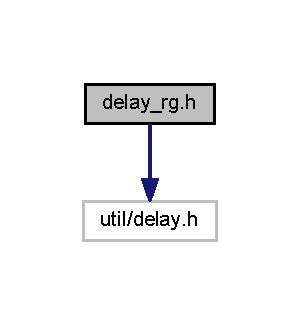
\includegraphics[width=144pt]{delay__rg_8h__incl}
\end{center}
\end{figure}
This graph shows which files directly or indirectly include this file\-:\nopagebreak
\begin{figure}[H]
\begin{center}
\leavevmode
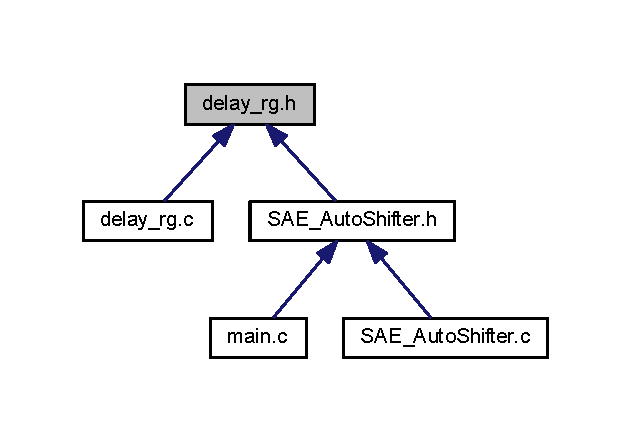
\includegraphics[width=303pt]{delay__rg_8h__dep__incl}
\end{center}
\end{figure}
\subsection*{Defines}
\begin{DoxyCompactItemize}
\item 
\hypertarget{delay__rg_8h_aa5f04ae75dc59a0cdd7ce0631acc3ae4}{\#define {\bfseries D\-L\-A\-Y\-\_\-\-M\-A\-X\-\_\-\-M\-S}~(262.\-14/F\-\_\-\-C\-P\-U)-\/1}\label{delay__rg_8h_aa5f04ae75dc59a0cdd7ce0631acc3ae4}

\item 
\hypertarget{delay__rg_8h_a8bf8812957a4b5dd27215dc9c12faf5f}{\#define {\bfseries D\-L\-A\-Y\-\_\-\-M\-A\-X\-\_\-\-U\-S}~(768/F\-\_\-\-C\-P\-U)-\/1}\label{delay__rg_8h_a8bf8812957a4b5dd27215dc9c12faf5f}

\end{DoxyCompactItemize}
\subsection*{Functions}
\begin{DoxyCompactItemize}
\item 
void \hyperlink{delay__rg_8h_aa0dce6d249d81fb85b082273270ba710}{delay\-\_\-ms} (uint16\-\_\-t ms)
\begin{DoxyCompactList}\small\item\em Delays for {\ttfamily ms} milliseconds. \end{DoxyCompactList}\item 
void \hyperlink{delay__rg_8h_a58f9378c36dbb864c00f8c964c652173}{delay\-\_\-us} (uint16\-\_\-t us)
\begin{DoxyCompactList}\small\item\em Delays for {\ttfamily us} microseconds. \end{DoxyCompactList}\end{DoxyCompactItemize}


\subsection{Detailed Description}
This file defines delay functions that extend the usefullness of the avr-\/gcc delay functions. \begin{DoxyAuthor}{Author}
Rocky Gray Jr.
\end{DoxyAuthor}
\begin{DoxyDate}{Date}
2/6/2012 
\end{DoxyDate}


\subsection{Function Documentation}
\hypertarget{delay__rg_8h_aa0dce6d249d81fb85b082273270ba710}{\index{delay\-\_\-rg.\-h@{delay\-\_\-rg.\-h}!delay\-\_\-ms@{delay\-\_\-ms}}
\index{delay\-\_\-ms@{delay\-\_\-ms}!delay_rg.h@{delay\-\_\-rg.\-h}}
\subsubsection[{delay\-\_\-ms}]{\setlength{\rightskip}{0pt plus 5cm}void {\bf delay\-\_\-ms} (
\begin{DoxyParamCaption}
\item[{uint16\-\_\-t}]{ms}
\end{DoxyParamCaption}
)}}\label{delay__rg_8h_aa0dce6d249d81fb85b082273270ba710}


Delays for {\ttfamily ms} milliseconds. 

Allows for longer delays. The longest delay that \-\_\-delay\-\_\-ms() can provide is 262.\-14ms / F\-\_\-\-C\-P\-U(in M\-Hz).


\begin{DoxyParams}{Parameters}
{\em ms} & length of delay in miliseconds \\
\hline
\end{DoxyParams}
\begin{DoxyReturn}{Returns}
none 
\end{DoxyReturn}
\hypertarget{delay__rg_8h_a58f9378c36dbb864c00f8c964c652173}{\index{delay\-\_\-rg.\-h@{delay\-\_\-rg.\-h}!delay\-\_\-us@{delay\-\_\-us}}
\index{delay\-\_\-us@{delay\-\_\-us}!delay_rg.h@{delay\-\_\-rg.\-h}}
\subsubsection[{delay\-\_\-us}]{\setlength{\rightskip}{0pt plus 5cm}void {\bf delay\-\_\-us} (
\begin{DoxyParamCaption}
\item[{uint16\-\_\-t}]{us}
\end{DoxyParamCaption}
)}}\label{delay__rg_8h_a58f9378c36dbb864c00f8c964c652173}


Delays for {\ttfamily us} microseconds. 

Allows for longer delays. The longest delay that \-\_\-delay\-\_\-us() can provide is 768us / F\-\_\-\-C\-P\-U(in M\-Hz).


\begin{DoxyParams}{Parameters}
{\em us} & length of delay in microseconds \\
\hline
\end{DoxyParams}
\begin{DoxyReturn}{Returns}
none 
\end{DoxyReturn}

\hypertarget{main_8c}{\section{main.\-c File Reference}
\label{main_8c}\index{main.\-c@{main.\-c}}
}


This file contains device specific initialization tasks and the main function.  


{\ttfamily \#include $<$stdio.\-h$>$}\\*
{\ttfamily \#include \char`\"{}S\-A\-E\-\_\-\-Auto\-Shifter.\-h\char`\"{}}\\*
{\ttfamily \#include \char`\"{}serial.\-h\char`\"{}}\\*
Include dependency graph for main.\-c\-:\nopagebreak
\begin{figure}[H]
\begin{center}
\leavevmode
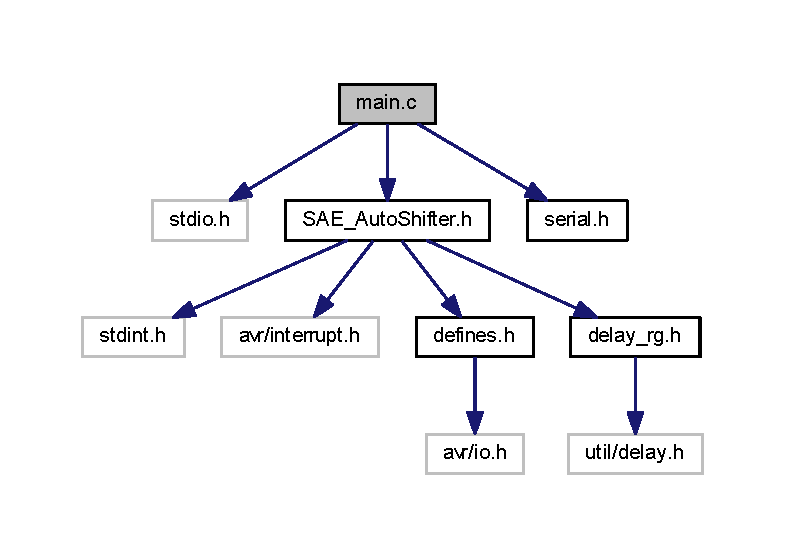
\includegraphics[width=350pt]{main_8c__incl}
\end{center}
\end{figure}
\subsection*{Defines}
\begin{DoxyCompactItemize}
\item 
\hypertarget{main_8c_a43bafb28b29491ec7f871319b5a3b2f8}{\#define {\bfseries F\-\_\-\-C\-P\-U}~16000000\-L}\label{main_8c_a43bafb28b29491ec7f871319b5a3b2f8}

\item 
\hypertarget{main_8c_ad72dbcf6d0153db1b8d8a58001feed83}{\#define \hyperlink{main_8c_ad72dbcf6d0153db1b8d8a58001feed83}{D\-E\-B\-U\-G}}\label{main_8c_ad72dbcf6d0153db1b8d8a58001feed83}

\begin{DoxyCompactList}\small\item\em Uncomment \hyperlink{main_8c_ad72dbcf6d0153db1b8d8a58001feed83}{D\-E\-B\-U\-G} to print out system information. \end{DoxyCompactList}\end{DoxyCompactItemize}
\subsection*{Functions}
\begin{DoxyCompactItemize}
\item 
void \hyperlink{main_8c_a43bba613ce0efd6af387cd04458ede8d}{io\-\_\-init} (void)
\begin{DoxyCompactList}\small\item\em Initialize i/o ports and timer. \end{DoxyCompactList}\item 
void \hyperlink{main_8c_a99ccbea44caa7d91c17782c602f956ef}{timer0\-\_\-init} (void)
\begin{DoxyCompactList}\small\item\em Initialize Timer 0. \end{DoxyCompactList}\item 
void \hyperlink{main_8c_a968c314be24f7043eeff034ebf7c4a03}{timer1\-\_\-init} (void)
\begin{DoxyCompactList}\small\item\em Initialize Timer 1. \end{DoxyCompactList}\item 
\hypertarget{main_8c_a840291bc02cba5474a4cb46a9b9566fe}{int \hyperlink{main_8c_a840291bc02cba5474a4cb46a9b9566fe}{main} (void)}\label{main_8c_a840291bc02cba5474a4cb46a9b9566fe}

\begin{DoxyCompactList}\small\item\em The main task for the autoshifter. \end{DoxyCompactList}\end{DoxyCompactItemize}
\subsection*{Variables}
\begin{DoxyCompactItemize}
\item 
uint8\-\_\-t \hyperlink{main_8c_a5b546e0fdb3a98f6a19d58c606431b88}{tick}
\begin{DoxyCompactList}\small\item\em Uncomment \#\-S\-I\-M\-U\-L\-A\-T\-E in order to use the rpm regulator simulation. \end{DoxyCompactList}\item 
\hypertarget{main_8c_a1da220fbb1464acf8ebf211ba8f942be}{uint8\-\_\-t \hyperlink{main_8c_a1da220fbb1464acf8ebf211ba8f942be}{can\-Print}}\label{main_8c_a1da220fbb1464acf8ebf211ba8f942be}

\begin{DoxyCompactList}\small\item\em D\-E\-B\-U\-G variable -\/ print flag. \end{DoxyCompactList}\end{DoxyCompactItemize}


\subsection{Detailed Description}
This file contains device specific initialization tasks and the main function. \begin{DoxySeeAlso}{See also}
\hyperlink{defines_8h}{defines.\-h} 
\end{DoxySeeAlso}
\begin{DoxyAuthor}{Author}
Rocky Gray Jr.
\end{DoxyAuthor}
\begin{DoxyDate}{Date}
3/11/2012 
\end{DoxyDate}


\subsection{Function Documentation}
\hypertarget{main_8c_a43bba613ce0efd6af387cd04458ede8d}{\index{main.\-c@{main.\-c}!io\-\_\-init@{io\-\_\-init}}
\index{io\-\_\-init@{io\-\_\-init}!main.c@{main.\-c}}
\subsubsection[{io\-\_\-init}]{\setlength{\rightskip}{0pt plus 5cm}void {\bf io\-\_\-init} (
\begin{DoxyParamCaption}
\item[{void}]{}
\end{DoxyParamCaption}
)\hspace{0.3cm}{\ttfamily  \mbox{[}inline\mbox{]}}}}\label{main_8c_a43bba613ce0efd6af387cd04458ede8d}


Initialize i/o ports and timer. 

\hypertarget{main_8c_init2}{}\subsection{Outputs\-:}\label{main_8c_init2}

\begin{DoxyItemize}
\item Solenoid Output
\begin{DoxyItemize}
\item \hyperlink{defines_8h_a3ca3b069d7464c17c03b5b1e7da788fd}{S\-O\-L\-E\-N\-\_\-\-O\-P\-\_\-\-D\-D\-R} =$>$ set \hyperlink{defines_8h_ae38dab54770629f5f2b7975164123353}{S\-O\-L\-E\-N\-\_\-\-D\-N} and \hyperlink{defines_8h_aeacdff688cfbf944da03e3c972f878f0}{S\-O\-L\-E\-N\-\_\-\-U\-P} as output
\item \hyperlink{defines_8h_a4ad600582a951bdd4b75311388dc6ae7}{S\-O\-L\-E\-N\-\_\-\-O\-P\-\_\-\-P\-O\-R\-T} =$>$ initialize \hyperlink{defines_8h_ae38dab54770629f5f2b7975164123353}{S\-O\-L\-E\-N\-\_\-\-D\-N} and \hyperlink{defines_8h_aeacdff688cfbf944da03e3c972f878f0}{S\-O\-L\-E\-N\-\_\-\-U\-P} to 0
\end{DoxyItemize}
\item Board Light Output
\begin{DoxyItemize}
\item \hyperlink{defines_8h_ae5ba1fb0b349f2a7f2fb82cb2cf39cbb}{B\-O\-A\-R\-D\-\_\-\-D\-D\-R} =$>$ set \hyperlink{defines_8h_a9ac61ad7c19d5a7d1f4cb1b45f41c7b1}{B\-O\-A\-R\-D\-\_\-\-L\-I\-G\-H\-T} as output
\item \hyperlink{defines_8h_a538e637dc4c2e333b294814e381d9a75}{B\-O\-A\-R\-D\-\_\-\-P\-O\-R\-T} =$>$ initialize B\-O\-A\-R\-D\-\_\-\-L\-I\-G\-H\-T to 0 
\end{DoxyItemize}
\end{DoxyItemize}\hypertarget{main_8c_init1}{}\subsection{Inputs\-:}\label{main_8c_init1}

\begin{DoxyItemize}
\item User Buttons
\begin{DoxyItemize}
\item \hyperlink{defines_8h_a0f1aed08f5269f1bddc80c20ecaec0be}{B\-T\-N\-\_\-\-I\-P\-\_\-\-D\-D\-R} =$>$ set \hyperlink{defines_8h_ac4a361c6ecdb8ef9a4c7a7253fa0feb8}{U\-S\-H\-I\-F\-T\-\_\-\-P\-I\-N} and \hyperlink{defines_8h_a7f2aeb6091a43ad2b243e35a521ec5b0}{D\-S\-H\-I\-F\-T\-\_\-\-P\-I\-N} as input
\item \hyperlink{defines_8h_a6ac943017d31877e3b86387e14c9b006}{B\-T\-N\-\_\-\-I\-P\-\_\-\-P\-O\-R\-T} =$>$ set pullups for \hyperlink{defines_8h_ac4a361c6ecdb8ef9a4c7a7253fa0feb8}{U\-S\-H\-I\-F\-T\-\_\-\-P\-I\-N} and \hyperlink{defines_8h_a7f2aeb6091a43ad2b243e35a521ec5b0}{D\-S\-H\-I\-F\-T\-\_\-\-P\-I\-N}
\end{DoxyItemize}
\item Tachometer Input
\begin{DoxyItemize}
\item \#\-T\-A\-C\-H\-\_\-\-I\-P\-\_\-\-D\-D\-R =$>$ set \hyperlink{defines_8h_af84d0d7a25d38271813b650eeb6a4228}{T\-A\-C\-H\-\_\-\-P\-I\-N} as input
\item Enable external Interrupt
\end{DoxyItemize}
\item Gas Pedal Input
\begin{DoxyItemize}
\item Enable A\-D\-C
\begin{DoxyItemize}
\item 128 Prescaler
\item A\-R\-E\-F = A\-V\-C\-C
\item Left align result
\item Free Running mode 
\end{DoxyItemize}
\end{DoxyItemize}
\end{DoxyItemize}\hypertarget{main_8c_a99ccbea44caa7d91c17782c602f956ef}{\index{main.\-c@{main.\-c}!timer0\-\_\-init@{timer0\-\_\-init}}
\index{timer0\-\_\-init@{timer0\-\_\-init}!main.c@{main.\-c}}
\subsubsection[{timer0\-\_\-init}]{\setlength{\rightskip}{0pt plus 5cm}void {\bf timer0\-\_\-init} (
\begin{DoxyParamCaption}
\item[{void}]{}
\end{DoxyParamCaption}
)\hspace{0.3cm}{\ttfamily  \mbox{[}inline\mbox{]}}}}\label{main_8c_a99ccbea44caa7d91c17782c602f956ef}


Initialize Timer 0. 

Timer 0\-:
\begin{DoxyItemize}
\item Configure Timer 0 for C\-T\-C (Clear Timer on Compare)
\item Prescaler set to \hyperlink{defines_8h_a42b5bcd9eeb1d25e27f7dffba04a1507}{P\-R\-E\-S\-C\-A\-L\-E\-R0} (16\-M\-Hz/\hyperlink{defines_8h_a42b5bcd9eeb1d25e27f7dffba04a1507}{P\-R\-E\-S\-C\-A\-L\-E\-R0})
\item Fires every \hyperlink{defines_8h_abbc7611d058a56c043591fab1ffede31}{T\-I\-M\-E\-R0\-\_\-\-F\-R\-E\-Q} Hz 
\end{DoxyItemize}\hypertarget{main_8c_a968c314be24f7043eeff034ebf7c4a03}{\index{main.\-c@{main.\-c}!timer1\-\_\-init@{timer1\-\_\-init}}
\index{timer1\-\_\-init@{timer1\-\_\-init}!main.c@{main.\-c}}
\subsubsection[{timer1\-\_\-init}]{\setlength{\rightskip}{0pt plus 5cm}void {\bf timer1\-\_\-init} (
\begin{DoxyParamCaption}
\item[{void}]{}
\end{DoxyParamCaption}
)\hspace{0.3cm}{\ttfamily  \mbox{[}inline\mbox{]}}}}\label{main_8c_a968c314be24f7043eeff034ebf7c4a03}


Initialize Timer 1. 

Timer 1\-:
\begin{DoxyItemize}
\item Configure Timer 1 for...
\item Prescaler set to \hyperlink{defines_8h_a8e5346fd5983419a0dbcbbc4995c7ea7}{P\-R\-E\-S\-C\-A\-L\-E\-R1} (16\-M\-Hz/\hyperlink{defines_8h_a8e5346fd5983419a0dbcbbc4995c7ea7}{P\-R\-E\-S\-C\-A\-L\-E\-R1})
\item Fires every \hyperlink{defines_8h_a2f78c07e3b43ef498e926a39eff06b04}{T\-I\-M\-E\-R1\-\_\-\-F\-R\-E\-Q} Hz 
\end{DoxyItemize}

\subsection{Variable Documentation}
\hypertarget{main_8c_a5b546e0fdb3a98f6a19d58c606431b88}{\index{main.\-c@{main.\-c}!tick@{tick}}
\index{tick@{tick}!main.c@{main.\-c}}
\subsubsection[{tick}]{\setlength{\rightskip}{0pt plus 5cm}uint8\-\_\-t {\bf tick}}}\label{main_8c_a5b546e0fdb3a98f6a19d58c606431b88}


Uncomment \#\-S\-I\-M\-U\-L\-A\-T\-E in order to use the rpm regulator simulation. 

D\-E\-B\-U\-G variable -\/ system tick 
\hypertarget{_s_a_e___auto_shifter_8c}{\section{S\-A\-E\-\_\-\-Auto\-Shifter.\-c File Reference}
\label{_s_a_e___auto_shifter_8c}\index{S\-A\-E\-\_\-\-Auto\-Shifter.\-c@{S\-A\-E\-\_\-\-Auto\-Shifter.\-c}}
}


This file defines the main task and I\-S\-Rs.  


{\ttfamily \#include \char`\"{}S\-A\-E\-\_\-\-Auto\-Shifter.\-h\char`\"{}}\\*
Include dependency graph for S\-A\-E\-\_\-\-Auto\-Shifter.\-c\-:\nopagebreak
\begin{figure}[H]
\begin{center}
\leavevmode
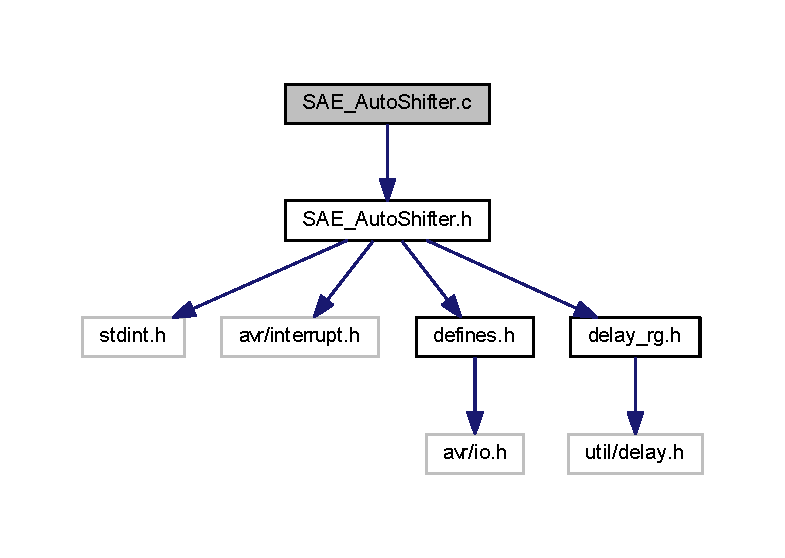
\includegraphics[width=350pt]{_s_a_e___auto_shifter_8c__incl}
\end{center}
\end{figure}
\subsection*{Functions}
\begin{DoxyCompactItemize}
\item 
\hyperlink{_s_a_e___auto_shifter_8c_aec43762dc86e029b395d4e5819192c2d}{I\-S\-R} (T\-I\-M\-E\-R0\-\_\-\-C\-O\-M\-P\-A\-\_\-vect)
\begin{DoxyCompactList}\small\item\em Update the button states. \end{DoxyCompactList}\item 
\hyperlink{_s_a_e___auto_shifter_8c_ad39420cdd896dd12c68e36313139d0a5}{I\-S\-R} (T\-I\-M\-E\-R1\-\_\-\-C\-O\-M\-P\-A\-\_\-vect)
\begin{DoxyCompactList}\small\item\em Tachometer sample time. \end{DoxyCompactList}\item 
\hyperlink{_s_a_e___auto_shifter_8c_afea150fcd685610cb9f7672fce361e53}{I\-S\-R} (I\-N\-T0\-\_\-vect)
\begin{DoxyCompactList}\small\item\em Count pulses from the tachometer. Fires at the rising edge of signal. \end{DoxyCompactList}\end{DoxyCompactItemize}


\subsection{Detailed Description}
This file defines the main task and I\-S\-Rs. \begin{DoxyAuthor}{Author}
Rocky Gray Jr.
\end{DoxyAuthor}
\begin{DoxyDate}{Date}
2/6/2012 
\end{DoxyDate}


\subsection{Function Documentation}
\hypertarget{_s_a_e___auto_shifter_8c_aec43762dc86e029b395d4e5819192c2d}{\index{S\-A\-E\-\_\-\-Auto\-Shifter.\-c@{S\-A\-E\-\_\-\-Auto\-Shifter.\-c}!I\-S\-R@{I\-S\-R}}
\index{I\-S\-R@{I\-S\-R}!SAE_AutoShifter.c@{S\-A\-E\-\_\-\-Auto\-Shifter.\-c}}
\subsubsection[{I\-S\-R}]{\setlength{\rightskip}{0pt plus 5cm}{\bf I\-S\-R} (
\begin{DoxyParamCaption}
\item[{T\-I\-M\-E\-R0\-\_\-\-C\-O\-M\-P\-A\-\_\-vect}]{}
\end{DoxyParamCaption}
)}}\label{_s_a_e___auto_shifter_8c_aec43762dc86e029b395d4e5819192c2d}


Update the button states. 

Fires at \hyperlink{defines_8h_abbc7611d058a56c043591fab1ffede31}{T\-I\-M\-E\-R0\-\_\-\-F\-R\-E\-Q} Hz. \hypertarget{_s_a_e___auto_shifter_8c_ad39420cdd896dd12c68e36313139d0a5}{\index{S\-A\-E\-\_\-\-Auto\-Shifter.\-c@{S\-A\-E\-\_\-\-Auto\-Shifter.\-c}!I\-S\-R@{I\-S\-R}}
\index{I\-S\-R@{I\-S\-R}!SAE_AutoShifter.c@{S\-A\-E\-\_\-\-Auto\-Shifter.\-c}}
\subsubsection[{I\-S\-R}]{\setlength{\rightskip}{0pt plus 5cm}{\bf I\-S\-R} (
\begin{DoxyParamCaption}
\item[{T\-I\-M\-E\-R1\-\_\-\-C\-O\-M\-P\-A\-\_\-vect}]{}
\end{DoxyParamCaption}
)}}\label{_s_a_e___auto_shifter_8c_ad39420cdd896dd12c68e36313139d0a5}


Tachometer sample time. 

Fires at \hyperlink{defines_8h_a2f78c07e3b43ef498e926a39eff06b04}{T\-I\-M\-E\-R1\-\_\-\-F\-R\-E\-Q} Hz. (1ms) \begin{DoxyParagraph}{Converts the number of pulses counted}
from the external interrupt into a value that represents the instantaneous rpms of the engine. It also places the current rpms into the history of rpms. 
\end{DoxyParagraph}
\hypertarget{_s_a_e___auto_shifter_8c_afea150fcd685610cb9f7672fce361e53}{\index{S\-A\-E\-\_\-\-Auto\-Shifter.\-c@{S\-A\-E\-\_\-\-Auto\-Shifter.\-c}!I\-S\-R@{I\-S\-R}}
\index{I\-S\-R@{I\-S\-R}!SAE_AutoShifter.c@{S\-A\-E\-\_\-\-Auto\-Shifter.\-c}}
\subsubsection[{I\-S\-R}]{\setlength{\rightskip}{0pt plus 5cm}{\bf I\-S\-R} (
\begin{DoxyParamCaption}
\item[{I\-N\-T0\-\_\-vect}]{}
\end{DoxyParamCaption}
)}}\label{_s_a_e___auto_shifter_8c_afea150fcd685610cb9f7672fce361e53}


Count pulses from the tachometer. Fires at the rising edge of signal. 

\begin{DoxyParagraph}{Counts the pulses from the tachometer until T\-I\-M\-E\-R1 fires.}

\end{DoxyParagraph}

\hypertarget{_s_a_e___auto_shifter_8h}{\section{S\-A\-E\-\_\-\-Auto\-Shifter.\-h File Reference}
\label{_s_a_e___auto_shifter_8h}\index{S\-A\-E\-\_\-\-Auto\-Shifter.\-h@{S\-A\-E\-\_\-\-Auto\-Shifter.\-h}}
}


This header file contains constant definitions and function prototypes.  


{\ttfamily \#include $<$stdint.\-h$>$}\\*
{\ttfamily \#include $<$avr/interrupt.\-h$>$}\\*
{\ttfamily \#include \char`\"{}defines.\-h\char`\"{}}\\*
{\ttfamily \#include \char`\"{}delay\-\_\-rg.\-h\char`\"{}}\\*
Include dependency graph for S\-A\-E\-\_\-\-Auto\-Shifter.\-h\-:\nopagebreak
\begin{figure}[H]
\begin{center}
\leavevmode
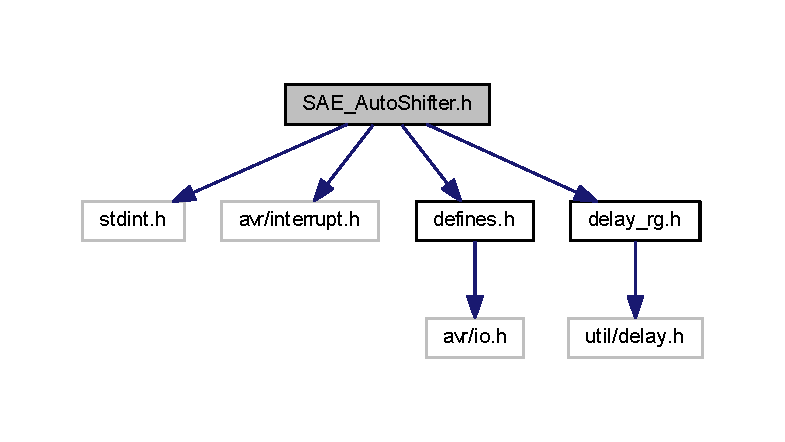
\includegraphics[width=350pt]{_s_a_e___auto_shifter_8h__incl}
\end{center}
\end{figure}
This graph shows which files directly or indirectly include this file\-:\nopagebreak
\begin{figure}[H]
\begin{center}
\leavevmode
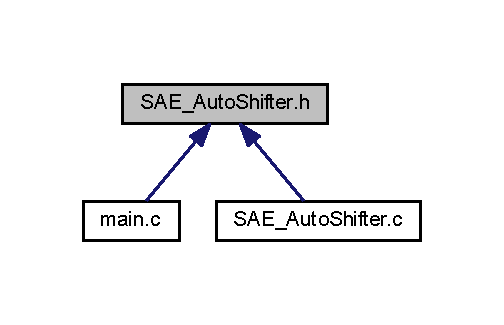
\includegraphics[width=242pt]{_s_a_e___auto_shifter_8h__dep__incl}
\end{center}
\end{figure}
\subsection*{Data Structures}
\begin{DoxyCompactItemize}
\item 
struct \hyperlink{struct_tach}{Tach}
\item 
struct \hyperlink{struct_usr___btns}{Usr\-\_\-\-Btns}
\item 
struct \hyperlink{struct_gear}{Gear}
\end{DoxyCompactItemize}
\subsection*{Enumerations}
\begin{DoxyCompactItemize}
\item 
enum \hyperlink{_s_a_e___auto_shifter_8h_a46c8a310cf4c094f8c80e1cb8dc1f911}{Mode} \{ {\bfseries manual}, 
{\bfseries semi\-\_\-man}, 
{\bfseries automated}
 \}
\begin{DoxyCompactList}\small\item\em Mode of the system. \end{DoxyCompactList}\end{DoxyCompactItemize}
\subsection*{Functions}
\begin{DoxyCompactItemize}
\item 
void \hyperlink{group__tacho_ga8746e3cc762f3153c2889e07dbb6ece0}{update\-\_\-ave\-\_\-rpms} ()
\item 
uint16\-\_\-t \hyperlink{group__tacho_gaa71ed50a06812b35c553b2291460396e}{average\-\_\-rpms} ()
\item 
\hypertarget{group__tacho_ga962c04c1da2810dd1602a83f649a454e}{uint16\-\_\-t {\bfseries cur\-\_\-rpms} ()}\label{group__tacho_ga962c04c1da2810dd1602a83f649a454e}

\item 
uint8\-\_\-t \hyperlink{group__usr_btns_ga12edd371195cb085c440d64794fdf9ea}{btn\-\_\-state} (\hyperlink{struct_usr___btns}{Usr\-\_\-\-Btns} $\ast$u\-\_\-btn)
\item 
uint16\-\_\-t \hyperlink{group__usr_btns_ga10ac2ecdef1d96d9ef177f948817bbb3}{btn\-\_\-count} (\hyperlink{struct_usr___btns}{Usr\-\_\-\-Btns} $\ast$u\-\_\-btn)
\item 
\hypertarget{group__usr_btns_ga2f0699e265a6cc26a98e3470366b5cda}{uint8\-\_\-t {\bfseries on\-Release} (\hyperlink{struct_usr___btns}{Usr\-\_\-\-Btns} $\ast$btn)}\label{group__usr_btns_ga2f0699e265a6cc26a98e3470366b5cda}

\item 
\hyperlink{_s_a_e___auto_shifter_8h_aec43762dc86e029b395d4e5819192c2d}{I\-S\-R} (T\-I\-M\-E\-R0\-\_\-\-C\-O\-M\-P\-A\-\_\-vect)
\begin{DoxyCompactList}\small\item\em Update the button states. \end{DoxyCompactList}\item 
\hyperlink{_s_a_e___auto_shifter_8h_ad39420cdd896dd12c68e36313139d0a5}{I\-S\-R} (T\-I\-M\-E\-R1\-\_\-\-C\-O\-M\-P\-A\-\_\-vect)
\begin{DoxyCompactList}\small\item\em Tachometer sample time. \end{DoxyCompactList}\item 
\hyperlink{_s_a_e___auto_shifter_8h_afea150fcd685610cb9f7672fce361e53}{I\-S\-R} (I\-N\-T0\-\_\-vect)
\begin{DoxyCompactList}\small\item\em Count pulses from the tachometer. Fires at the rising edge of signal. \end{DoxyCompactList}\end{DoxyCompactItemize}
\subsection*{Variables}
\begin{DoxyCompactItemize}
\item 
\hypertarget{_s_a_e___auto_shifter_8h_ab50f3f7ed3b6b9ab1fa2605b587eece5}{uint16\-\_\-t \hyperlink{_s_a_e___auto_shifter_8h_ab50f3f7ed3b6b9ab1fa2605b587eece5}{isr\-Count}}\label{_s_a_e___auto_shifter_8h_ab50f3f7ed3b6b9ab1fa2605b587eece5}

\begin{DoxyCompactList}\small\item\em I\-S\-R count. \end{DoxyCompactList}\item 
\hypertarget{_s_a_e___auto_shifter_8h_a5b546e0fdb3a98f6a19d58c606431b88}{uint8\-\_\-t \hyperlink{_s_a_e___auto_shifter_8h_a5b546e0fdb3a98f6a19d58c606431b88}{tick}}\label{_s_a_e___auto_shifter_8h_a5b546e0fdb3a98f6a19d58c606431b88}

\begin{DoxyCompactList}\small\item\em D\-E\-B\-U\-G variable -\/ system tick. \end{DoxyCompactList}\item 
uint8\-\_\-t \hyperlink{_s_a_e___auto_shifter_8h_a1da220fbb1464acf8ebf211ba8f942be}{can\-Print}
\item 
\hypertarget{_s_a_e___auto_shifter_8h_a325783c7ea3d1eaaf66a1c7bae56167b}{enum \hyperlink{_s_a_e___auto_shifter_8h_a46c8a310cf4c094f8c80e1cb8dc1f911}{Mode} \hyperlink{_s_a_e___auto_shifter_8h_a325783c7ea3d1eaaf66a1c7bae56167b}{mode}}\label{_s_a_e___auto_shifter_8h_a325783c7ea3d1eaaf66a1c7bae56167b}

\begin{DoxyCompactList}\small\item\em Mode switch. \end{DoxyCompactList}\item 
\hypertarget{group__tacho_ga3920911d3598cb499db825e8cb9adcad}{\hyperlink{struct_tach}{Tach} \hyperlink{group__tacho_ga3920911d3598cb499db825e8cb9adcad}{tach}}\label{group__tacho_ga3920911d3598cb499db825e8cb9adcad}

\begin{DoxyCompactList}\small\item\em Tachometer object. \end{DoxyCompactList}\item 
\hypertarget{group__usr_btns_ga18ee634a9df9ed1ca0c7af2e021cec0f}{\hyperlink{struct_usr___btns}{Usr\-\_\-\-Btns} \hyperlink{group__usr_btns_ga18ee634a9df9ed1ca0c7af2e021cec0f}{up\-\_\-shift}}\label{group__usr_btns_ga18ee634a9df9ed1ca0c7af2e021cec0f}

\begin{DoxyCompactList}\small\item\em Upshift button. \end{DoxyCompactList}\item 
\hypertarget{group__usr_btns_gafd0b4b5ca080e04e71e4308414dc58ed}{\hyperlink{struct_usr___btns}{Usr\-\_\-\-Btns} \hyperlink{group__usr_btns_gafd0b4b5ca080e04e71e4308414dc58ed}{dn\-\_\-shift}}\label{group__usr_btns_gafd0b4b5ca080e04e71e4308414dc58ed}

\begin{DoxyCompactList}\small\item\em Downshift button. \end{DoxyCompactList}\end{DoxyCompactItemize}
\begin{DoxyCompactItemize}
\item 
typedef struct \hyperlink{struct_gear}{Gear} \hyperlink{_s_a_e___auto_shifter_8h_a847ee2f4a6c9a7af8ca2cab32b5917be}{Gear}
\item 
\hypertarget{_s_a_e___auto_shifter_8h_a26fea787ee1628dff57b862089c4523b}{\hyperlink{struct_gear}{Gear} $\ast$ \hyperlink{_s_a_e___auto_shifter_8h_a26fea787ee1628dff57b862089c4523b}{gear\-\_\-}}\label{_s_a_e___auto_shifter_8h_a26fea787ee1628dff57b862089c4523b}

\begin{DoxyCompactList}\small\item\em Current gear. \end{DoxyCompactList}\item 
\hypertarget{_s_a_e___auto_shifter_8h_abf8478276f1c8d0a00333ad9f061b2e7}{void {\bfseries Gear\-\_\-\-Construct} (\hyperlink{struct_gear}{Gear} $\ast$this, uint8\-\_\-t num, uint16\-\_\-t lower, uint16\-\_\-t upper, \hyperlink{struct_gear}{Gear} $\ast$p, \hyperlink{struct_gear}{Gear} $\ast$n)}\label{_s_a_e___auto_shifter_8h_abf8478276f1c8d0a00333ad9f061b2e7}

\item 
uint8\-\_\-t \hyperlink{_s_a_e___auto_shifter_8h_adde353caf7da095b13aeb74c2cc31277}{gear\-\_\-num} ()
\item 
uint16\-\_\-t \hyperlink{_s_a_e___auto_shifter_8h_a3a18aa2ddacbcd7f3c5f6c48f8c813b3}{gear\-\_\-upper} ()
\item 
uint16\-\_\-t \hyperlink{_s_a_e___auto_shifter_8h_a1805be701915c837c3a779f8679d1701}{gear\-\_\-lower} ()
\item 
\hypertarget{_s_a_e___auto_shifter_8h_ab255f19ddfec9d8967d83c340c29de9e}{void {\bfseries shift} (uint8\-\_\-t direction)}\label{_s_a_e___auto_shifter_8h_ab255f19ddfec9d8967d83c340c29de9e}

\end{DoxyCompactItemize}


\subsection{Detailed Description}
This header file contains constant definitions and function prototypes. This project uses the Arduino Uno board. It uses the A\-T\-M\-E\-G\-A 328\-P microcontroller with a 16\-M\-Hz crystal oscillator. Pin mappings described below should only be used for this board or ones with the same pin mappings

\begin{DoxyAuthor}{Author}
Rocky Gray Jr.
\end{DoxyAuthor}
\begin{DoxyDate}{Date}
3/7/2012 
\end{DoxyDate}


\subsection{Typedef Documentation}
\hypertarget{_s_a_e___auto_shifter_8h_a847ee2f4a6c9a7af8ca2cab32b5917be}{\index{S\-A\-E\-\_\-\-Auto\-Shifter.\-h@{S\-A\-E\-\_\-\-Auto\-Shifter.\-h}!Gear@{Gear}}
\index{Gear@{Gear}!SAE_AutoShifter.h@{S\-A\-E\-\_\-\-Auto\-Shifter.\-h}}
\subsubsection[{Gear}]{\setlength{\rightskip}{0pt plus 5cm}n Next {\bf Gear}}}\label{_s_a_e___auto_shifter_8h_a847ee2f4a6c9a7af8ca2cab32b5917be}
defgroup gears Gears Defines the gear structure and related functions. 

\subsection{Function Documentation}
\hypertarget{_s_a_e___auto_shifter_8h_a1805be701915c837c3a779f8679d1701}{\index{S\-A\-E\-\_\-\-Auto\-Shifter.\-h@{S\-A\-E\-\_\-\-Auto\-Shifter.\-h}!gear\-\_\-lower@{gear\-\_\-lower}}
\index{gear\-\_\-lower@{gear\-\_\-lower}!SAE_AutoShifter.h@{S\-A\-E\-\_\-\-Auto\-Shifter.\-h}}
\subsubsection[{gear\-\_\-lower}]{\setlength{\rightskip}{0pt plus 5cm}uint16\-\_\-t {\bf gear\-\_\-lower} (
\begin{DoxyParamCaption}
{}
\end{DoxyParamCaption}
)\hspace{0.3cm}{\ttfamily  \mbox{[}inline\mbox{]}}}}\label{_s_a_e___auto_shifter_8h_a1805be701915c837c3a779f8679d1701}
\hyperlink{_s_a_e___auto_shifter_8h_a1805be701915c837c3a779f8679d1701}{gear\-\_\-lower()}

\begin{DoxyReturn}{Returns}
The lower bound of the current gear 
\end{DoxyReturn}
\hypertarget{_s_a_e___auto_shifter_8h_adde353caf7da095b13aeb74c2cc31277}{\index{S\-A\-E\-\_\-\-Auto\-Shifter.\-h@{S\-A\-E\-\_\-\-Auto\-Shifter.\-h}!gear\-\_\-num@{gear\-\_\-num}}
\index{gear\-\_\-num@{gear\-\_\-num}!SAE_AutoShifter.h@{S\-A\-E\-\_\-\-Auto\-Shifter.\-h}}
\subsubsection[{gear\-\_\-num}]{\setlength{\rightskip}{0pt plus 5cm}uint8\-\_\-t {\bf gear\-\_\-num} (
\begin{DoxyParamCaption}
{}
\end{DoxyParamCaption}
)\hspace{0.3cm}{\ttfamily  \mbox{[}inline\mbox{]}}}}\label{_s_a_e___auto_shifter_8h_adde353caf7da095b13aeb74c2cc31277}
\hyperlink{_s_a_e___auto_shifter_8h_adde353caf7da095b13aeb74c2cc31277}{gear\-\_\-num()}

\begin{DoxyReturn}{Returns}
the number of the current gear 
\end{DoxyReturn}
\hypertarget{_s_a_e___auto_shifter_8h_a3a18aa2ddacbcd7f3c5f6c48f8c813b3}{\index{S\-A\-E\-\_\-\-Auto\-Shifter.\-h@{S\-A\-E\-\_\-\-Auto\-Shifter.\-h}!gear\-\_\-upper@{gear\-\_\-upper}}
\index{gear\-\_\-upper@{gear\-\_\-upper}!SAE_AutoShifter.h@{S\-A\-E\-\_\-\-Auto\-Shifter.\-h}}
\subsubsection[{gear\-\_\-upper}]{\setlength{\rightskip}{0pt plus 5cm}uint16\-\_\-t {\bf gear\-\_\-upper} (
\begin{DoxyParamCaption}
{}
\end{DoxyParamCaption}
)\hspace{0.3cm}{\ttfamily  \mbox{[}inline\mbox{]}}}}\label{_s_a_e___auto_shifter_8h_a3a18aa2ddacbcd7f3c5f6c48f8c813b3}
\hyperlink{_s_a_e___auto_shifter_8h_a3a18aa2ddacbcd7f3c5f6c48f8c813b3}{gear\-\_\-upper()}

\begin{DoxyReturn}{Returns}
The upper bound of the current gear 
\end{DoxyReturn}
\hypertarget{_s_a_e___auto_shifter_8h_aec43762dc86e029b395d4e5819192c2d}{\index{S\-A\-E\-\_\-\-Auto\-Shifter.\-h@{S\-A\-E\-\_\-\-Auto\-Shifter.\-h}!I\-S\-R@{I\-S\-R}}
\index{I\-S\-R@{I\-S\-R}!SAE_AutoShifter.h@{S\-A\-E\-\_\-\-Auto\-Shifter.\-h}}
\subsubsection[{I\-S\-R}]{\setlength{\rightskip}{0pt plus 5cm}{\bf I\-S\-R} (
\begin{DoxyParamCaption}
\item[{T\-I\-M\-E\-R0\-\_\-\-C\-O\-M\-P\-A\-\_\-vect}]{}
\end{DoxyParamCaption}
)}}\label{_s_a_e___auto_shifter_8h_aec43762dc86e029b395d4e5819192c2d}


Update the button states. 

Fires at \hyperlink{defines_8h_abbc7611d058a56c043591fab1ffede31}{T\-I\-M\-E\-R0\-\_\-\-F\-R\-E\-Q} Hz. \hypertarget{_s_a_e___auto_shifter_8h_ad39420cdd896dd12c68e36313139d0a5}{\index{S\-A\-E\-\_\-\-Auto\-Shifter.\-h@{S\-A\-E\-\_\-\-Auto\-Shifter.\-h}!I\-S\-R@{I\-S\-R}}
\index{I\-S\-R@{I\-S\-R}!SAE_AutoShifter.h@{S\-A\-E\-\_\-\-Auto\-Shifter.\-h}}
\subsubsection[{I\-S\-R}]{\setlength{\rightskip}{0pt plus 5cm}{\bf I\-S\-R} (
\begin{DoxyParamCaption}
\item[{T\-I\-M\-E\-R1\-\_\-\-C\-O\-M\-P\-A\-\_\-vect}]{}
\end{DoxyParamCaption}
)}}\label{_s_a_e___auto_shifter_8h_ad39420cdd896dd12c68e36313139d0a5}


Tachometer sample time. 

Fires at \hyperlink{defines_8h_a2f78c07e3b43ef498e926a39eff06b04}{T\-I\-M\-E\-R1\-\_\-\-F\-R\-E\-Q} Hz. (1ms) \begin{DoxyParagraph}{Converts the number of pulses counted}
from the external interrupt into a value that represents the instantaneous rpms of the engine. It also places the current rpms into the history of rpms. 
\end{DoxyParagraph}
\hypertarget{_s_a_e___auto_shifter_8h_afea150fcd685610cb9f7672fce361e53}{\index{S\-A\-E\-\_\-\-Auto\-Shifter.\-h@{S\-A\-E\-\_\-\-Auto\-Shifter.\-h}!I\-S\-R@{I\-S\-R}}
\index{I\-S\-R@{I\-S\-R}!SAE_AutoShifter.h@{S\-A\-E\-\_\-\-Auto\-Shifter.\-h}}
\subsubsection[{I\-S\-R}]{\setlength{\rightskip}{0pt plus 5cm}{\bf I\-S\-R} (
\begin{DoxyParamCaption}
\item[{I\-N\-T0\-\_\-vect}]{}
\end{DoxyParamCaption}
)}}\label{_s_a_e___auto_shifter_8h_afea150fcd685610cb9f7672fce361e53}


Count pulses from the tachometer. Fires at the rising edge of signal. 

\begin{DoxyParagraph}{Counts the pulses from the tachometer until T\-I\-M\-E\-R1 fires.}

\end{DoxyParagraph}


\subsection{Variable Documentation}
\hypertarget{_s_a_e___auto_shifter_8h_a1da220fbb1464acf8ebf211ba8f942be}{\index{S\-A\-E\-\_\-\-Auto\-Shifter.\-h@{S\-A\-E\-\_\-\-Auto\-Shifter.\-h}!can\-Print@{can\-Print}}
\index{can\-Print@{can\-Print}!SAE_AutoShifter.h@{S\-A\-E\-\_\-\-Auto\-Shifter.\-h}}
\subsubsection[{can\-Print}]{\setlength{\rightskip}{0pt plus 5cm}uint8\-\_\-t {\bf can\-Print}}}\label{_s_a_e___auto_shifter_8h_a1da220fbb1464acf8ebf211ba8f942be}
D\-E\-B\-U\-G variable -\/ print flag 
\printindex
\end{document}
